\documentclass[handout]{beamer} %handout para imprimir
\usetheme{Frankfurt}
\useoutertheme[subsection=false]{miniframes}
\usecolortheme{seahorse}
\usenavigationsymbolstemplate{}

\usepackage{color}
\usepackage{listings}
\usepackage[spanish]{babel}
\usepackage[utf8]{inputenc}
\usepackage{graphicx}
\usepackage{hyperref}
\usepackage{siunitx}
\usepackage[version=3]{mhchem}
\usepackage{multicol}
\usepackage{biblatex}
 
\title{Estudio de los Mecanismos Básicos de Electroporación a Través de la\\ Modelación Numérica}

\subtitle{Trabajo para optar por el título de\\ Licenciado en Ciencias de la Computación}

\author{Mauricio Alfonso}
\institute{Departamento de Computación\\ Facultad de Ciencias Exactas y Naturales - Universidad de Buenos Aires}
\date{11 de mayo de 2015}

\begin{document}

\sisetup{per-mode = symbol}
\newcommand{\h}{\ce{H^+}}
\newcommand{\oh}{\ce{OH^-}}
\newcommand{\na}{\ce{Na^+}}
\newcommand{\cl}{\ce{Cl^-}}
\newcommand{\ontime}{\texttt{ON TIME}}
\newcommand{\offtime}{\texttt{OFF TIME}}
	
\frame {
	\titlepage
}

%TODO cambiar el estilo! (que no quede subsection empty)

\section{Introducción} 

%\subsection{Introducción} 

\frame {
	%acá habría que poner algo basado en la introducción
	\frametitle{Electroporación}
	\begin{itemize}
		\item La \textbf{Electroporación} o \textbf{Electropermeabilización (EP)} consiste en la aplicación de pulsos eléctricos a una membrana biológica con el objetivo de incrementar su permeabilidad.
		\item De esta manera se facilita el ingreso de agentes terapéuticos a una célula.
		\item En la medicina se utiliza EP en la electroquimioterapia (ECT), la electrotransferencia génica (GET) y la electroporación irreversible (IRE).
		\item También tiene aplicaciones en el procesamiento de alimentos y la gestión ambiental. 
	\end{itemize}
}

\frame {
	% qué se hace y 4 partes
	\frametitle{Modelo}	
	
	En esta tesis se simula numéricamente la aplicación de pulsos eléctricos a un dominio que contiene a una célula y se estudia su respuesta eléctrica, la permeabilización lograda y el transporte de especies iónicas. 
	
	\vspace{\baselineskip}

	Se estudiaron tres tipos de fenómenos físicos por separado:

	\begin{itemize}
		\item El potencial eléctrico en todo el dominio \pause
		\item La creación y evolución de poros en la membrana celular \pause
		\item El transporte de especies iónicas \pause
	\end{itemize}
	
	Por último se analizaron todos los fenómenos acoplados.\\
}

\frame {
%	\frametitle{Dominio}
	\frametitle{Modelo}		
	
	\begin{columns}[c]
		\begin{column}{0.60\textwidth}
			\center{Dominio:\\}
			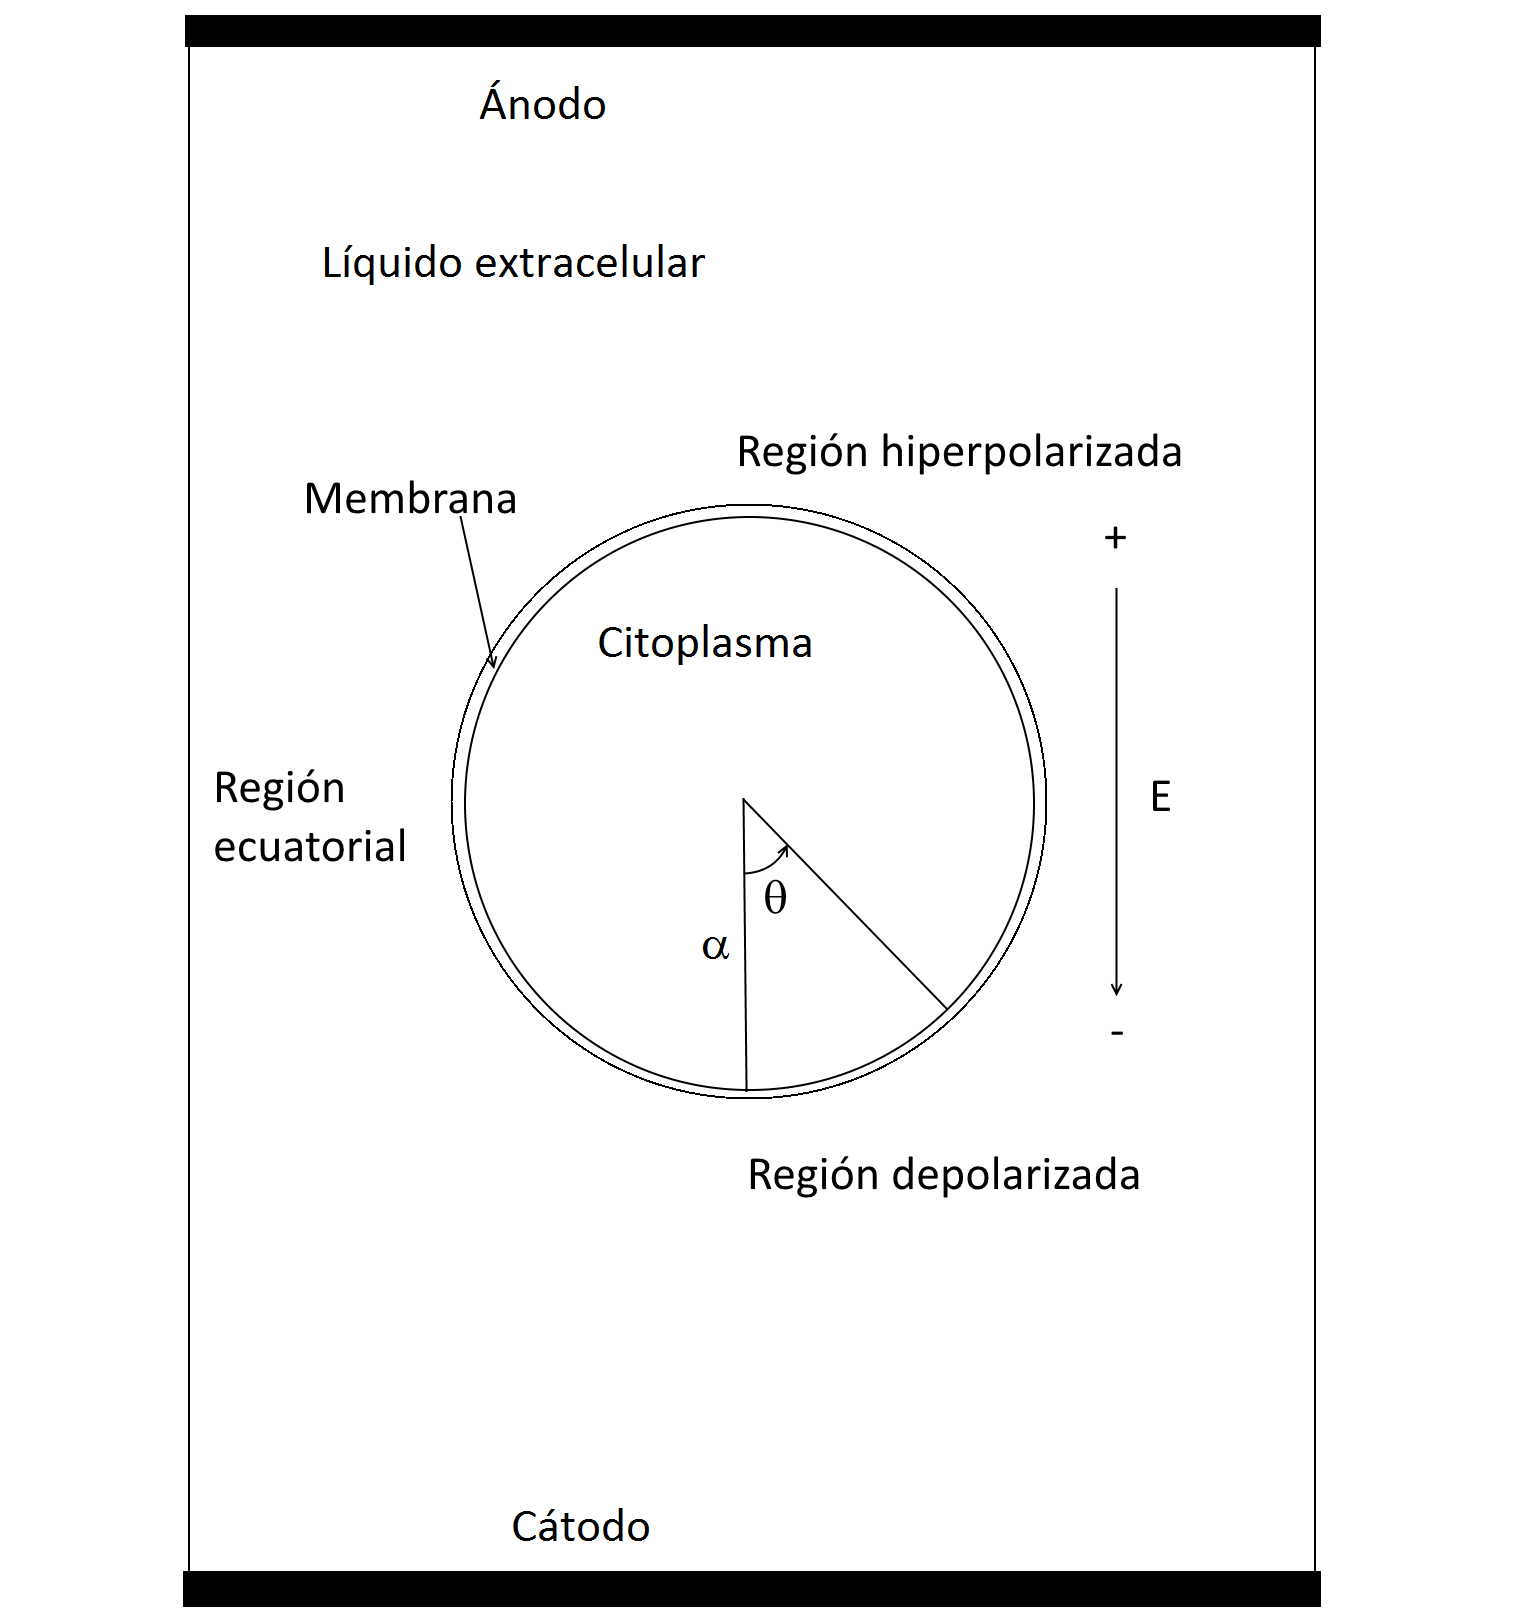
\includegraphics[width=1.0\textwidth]{graficos/dominio}
		\end{column}
		%\pause
		\begin{column}{0.50\textwidth}
			\center{Pulso:\\}
			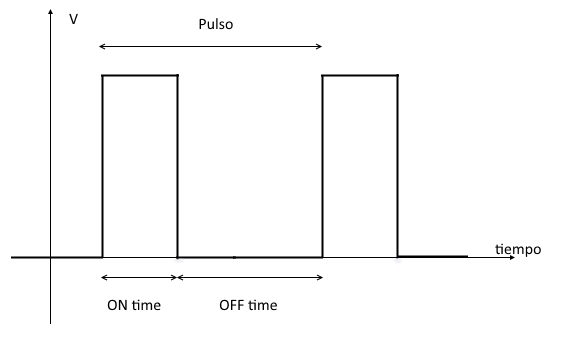
\includegraphics[width=1.0\textwidth]{graficos/pulso}
		\end{column}
	\end{columns}
}

\frame {
	\frametitle{Detalles}
	\begin{itemize}
		\item Células esféricas de entre 10 y 50 \si{\micro\metre} de radio.\footfullcite{Biophysical journal, 92(2), 404-417, 2007}\textsuperscript{,} \footfullcite{Annals of biomedical engineering, 34(4), 642-652, 2006} \pause
		\item Membrana celular de 5 \si{\nano\metre} de espesor.\footfullcite{Bioelectrochemistry 82, 10-21, 2011} \pause
		\item Pulsos eléctricos de pocos milisegundos de duración, que generan campos de hasta 2000 \si{\volt\per\centi\metre}. \footfullcite{Biophysical journal, 98(11), 2506-2514, 2010}\pause		
		\item Se considera un modelo donde la densidad de poros en la membrana celular y sus radios dependen del potencial transmembrana.$^{1}$\pause
		\item Se estudia la evolución de la concentración de 4 especies iónicas: \h, \oh, \na{} y \cl.
	\end{itemize}
}

\section{Implementación}

%\subsection{Métodos computacionales} 

\frame {
	%Mencionar FEM, Euler, C++, Eigen, OpenMP
	\frametitle{Métodos Computacionales}
	\begin{itemize}
		\item Se implementaron las simulaciones desde cero en \textbf{C\raisebox{.25ex}{++}}.
		\pause
		\item Se utiliza principalmente el \textbf{Método de Elementos Finitos} y en menor medida diferencias finitas.
		\pause
		\item Se modela la membrana explícitamente, en lugar de considerarla una condición de borde.
		\pause
		\item Se trabaja en un dominio bidimensional con coordenadas cilíndricas.
		\pause
		\item Se hizo uso de la biblioteca de álgebra lineal \textbf{Eigen} para \texttt{C++}.
		\pause		
		\item Descomposiciones \textbf{BiCGSTAB} y \textbf{LDL} con matrices esparsas para resolver los sistemas de ecuaciones del método de elementos finitos. 
		\pause		
		\item Se paralelizaron partes del código en varios hilos con \textbf{OpenMP}.
		\pause
		\item Adicionalmente se utilizó \textbf{Python} y la biblioteca \textbf{matplotlib} para procesar las salidas. 
	\end{itemize}
}

%\subsection{Mallado} 

\frame {
	%Poner imágenes y explicar.
	\frametitle{Mallado}
	\begin{multicols}{2}
		\itemize{
			\item Coordenadas cilíndricas (2D)
			\item Elementos cuadrilaterales
			\item Tamaño variable de los elementos
			\item Generadas con AutoMesh2D
			\item Entre 7000 y 9000 elementos según la malla
			\vspace{1cm}
		}
		\columnbreak
		\begin{center}
			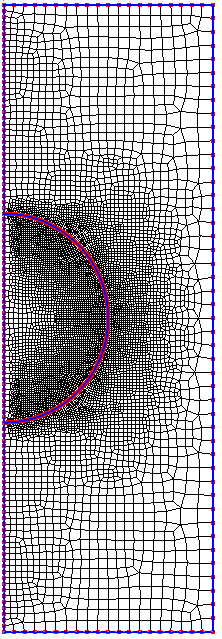
\includegraphics[keepaspectratio, height=0.85\textheight]{graficos/meshfar} \\
		\end{center}
	\end{multicols}
}

\frame {
	\frametitle{Mallado (detalle)}
	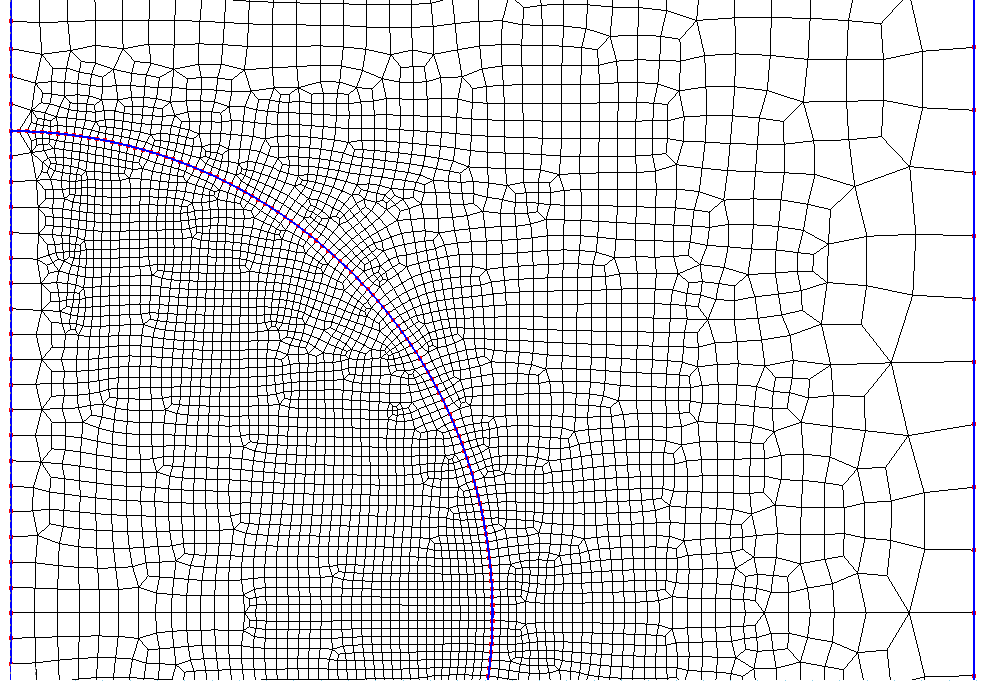
\includegraphics[width=\textwidth]{graficos/meshclose}
}

\frame {
	\frametitle{Mallado (membrana)}
	La membrana se modela explícitamente en la malla con dos elementos de ancho en la dirección radial. \\
	\vspace{0.25\baselineskip}
	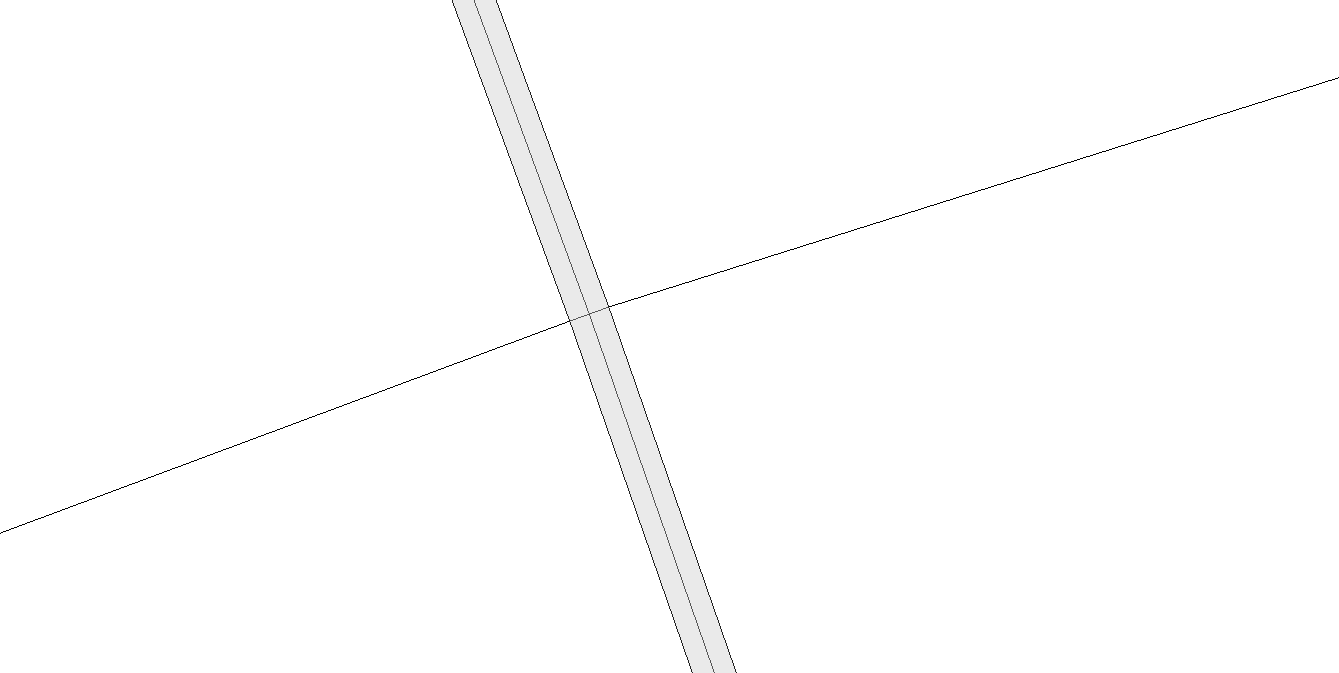
\includegraphics[width=\textwidth]{graficos/meshmembrane}
}

\section{Potencial Eléctrico}

%\subsection{Teoría} 

\frame {
	%Fórmulas
	\frametitle{Potencial Eléctrico}
	Ecuación de Poisson:
	\begin{equation*}
		\nabla ( \sigma_{elem} \cdot \nabla \phi) = 0 
	\end{equation*} \pause
	
	Condiciones de borde de Dirichlet en los electrodos y de Neumann en el borde restante. \pause
	
	\vspace{\baselineskip}
	La solución analítica del potencial transmembrana (PTM) puede aproximarse como:
	\begin{equation*}
		 PTM^{\theta} = f_s\, E\, \alpha\, \cos (\theta)
	\end{equation*}
}

%\subsection{Resultados} 

\frame {
	%Potencial eléctrico en el dominio
	\frametitle{Potencial Eléctrico}
%	\center{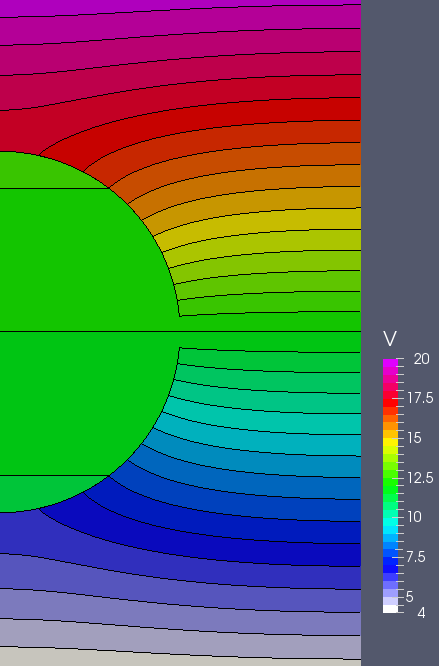
\includegraphics[height=0.80\textheight]{graficos/lineas}}
	
	\begin{multicols}{2}
		\center{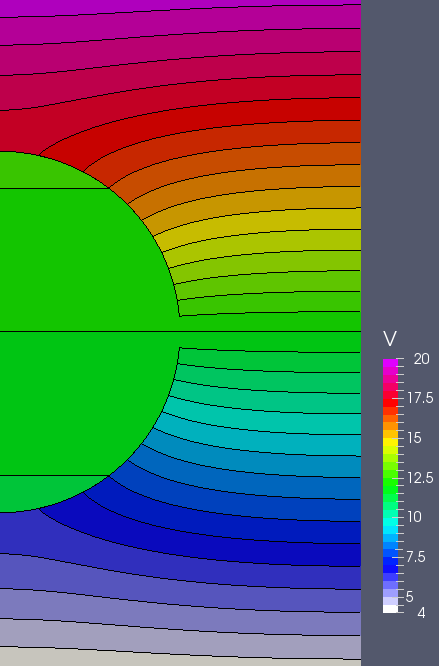
\includegraphics[height=0.85\textheight]{graficos/lineas}}\\
		\columnbreak
		Ejemplo para E = 1600 \si{\volt\per\centi\metre}\\ 
		$\alpha$ = 25 \si{\micro\metre}\\
		$\sigma_o$ = 0.20 \si{\siemens\per\metre}\\
		$\sigma_i$ = 0.15 \si{\siemens\per\metre}\\
		$\sigma_m$ = \num{5e-6} \si{\siemens\per\metre}\\
	\end{multicols}
}

\frame {
	\frametitle{Campo eléctrico (componente horizontal)}
	\begin{multicols}{2}
		\center{En el exterior:}
		\center{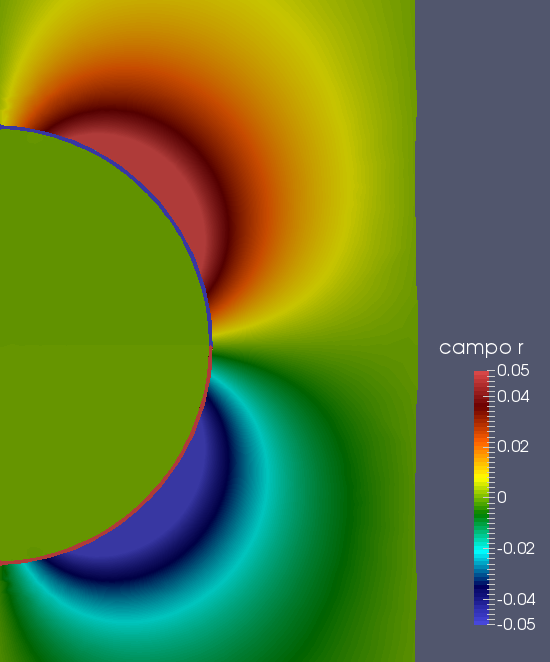
\includegraphics[width=0.45\textwidth]{graficos/campo-r}}\\
		\columnbreak
		\pause
		\center{En el interior:}
		\center{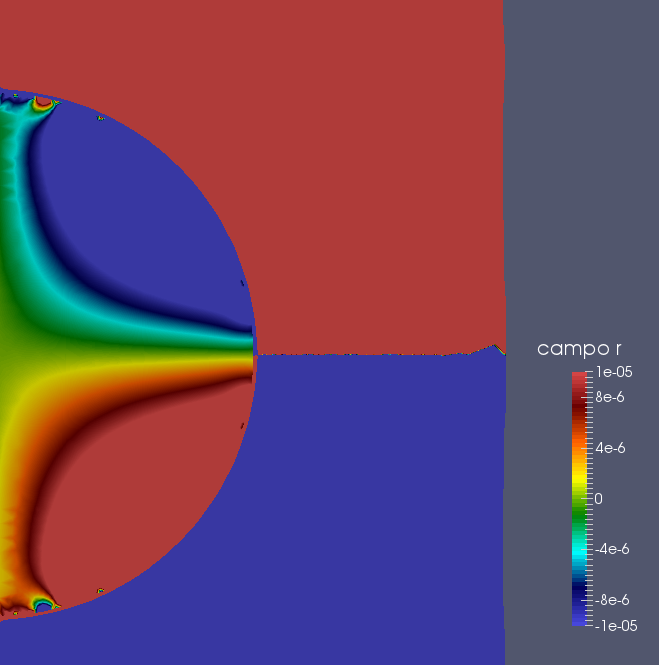
\includegraphics[width=0.45\textwidth]{graficos/campo-r-int}}
	\end{multicols}
}

\frame {
	\frametitle{Campo eléctrico (componente vertical)}
	\begin{multicols}{2}
		\center{En el exterior:}
		\center{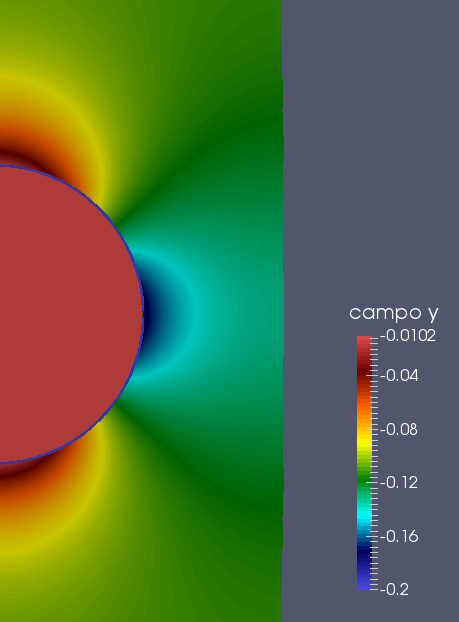
\includegraphics[width=0.45\textwidth]{graficos/campo-y}}\\
		\pause
		\columnbreak
		\center{En el interior:}
		\center{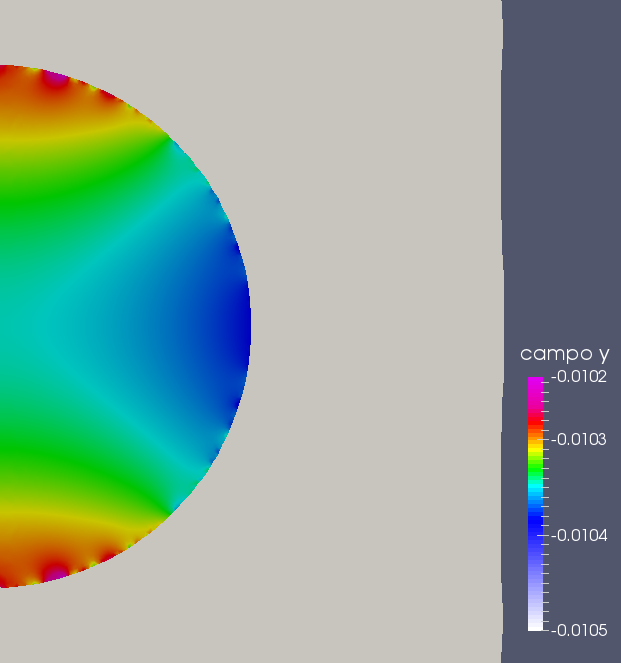
\includegraphics[width=0.45\textwidth]{graficos/campo-y-int}}
	\end{multicols}
}

\frame {
	\frametitle{Campo eléctrico (módulo)}
	\begin{multicols}{2}
		\center{En el exterior:}
		\center{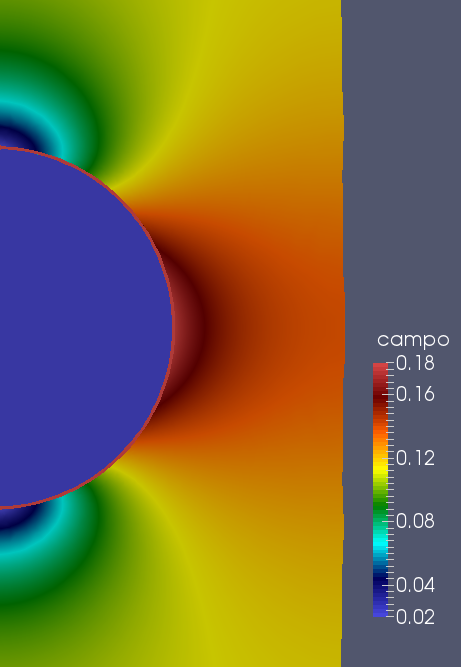
\includegraphics[width=0.40\textwidth]{graficos/campo}}\\
		\columnbreak
		\pause
		\center{En el interior:}
		\center{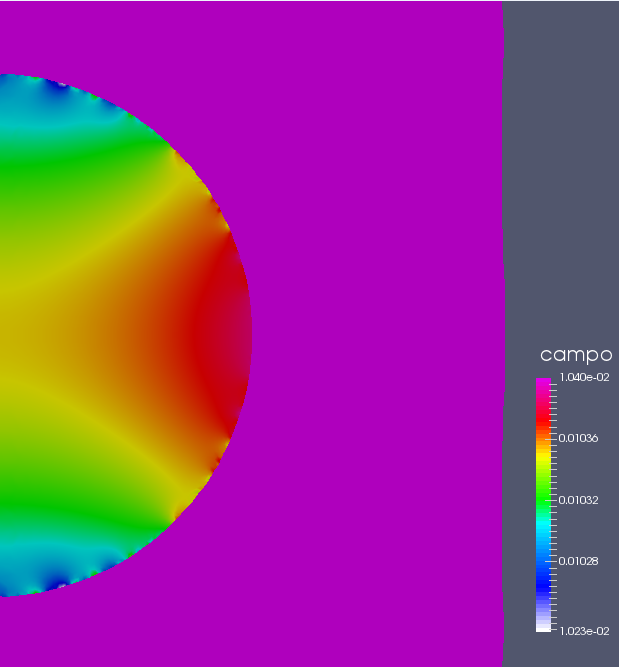
\includegraphics[width=0.45\textwidth]{graficos/campo-int}}
	\end{multicols}
}

\frame {
	\frametitle{Potencial Transmembrana}
	\begin{multicols}{2}
		\center{Para diferentes radios:}
		\center{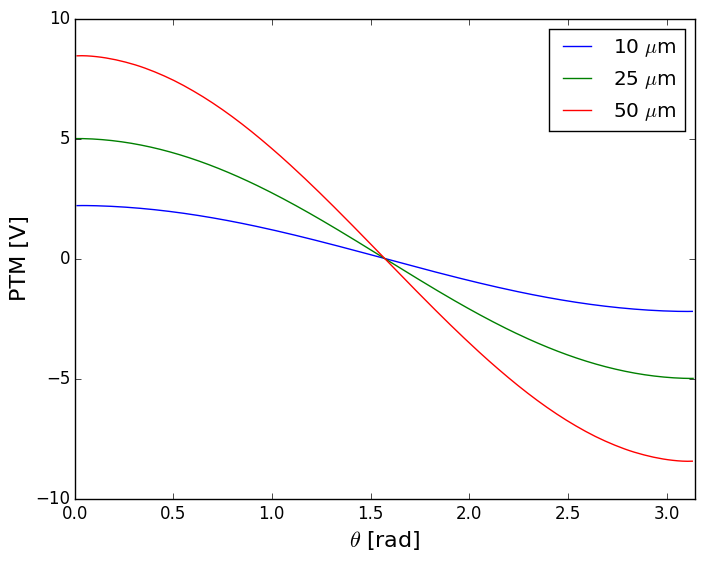
\includegraphics[width=0.50\textwidth]{graficos/itv-radio}}\\
		\columnbreak
		\pause
		\center{Para diferentes potenciales aplicados:}
		\center{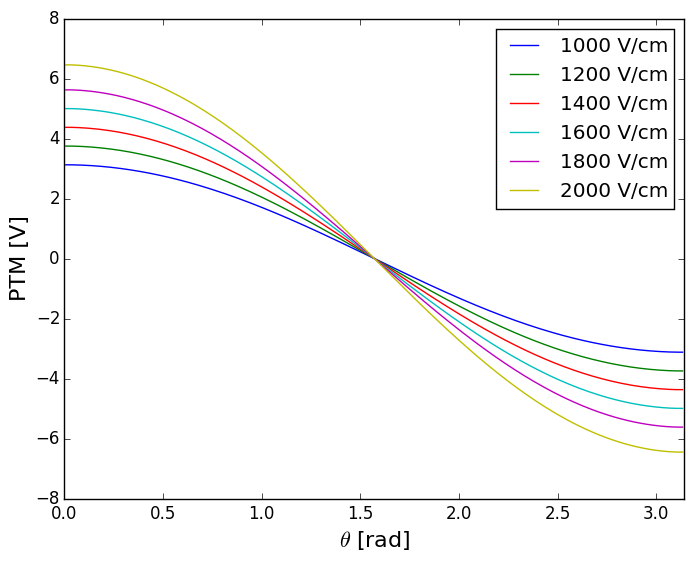
\includegraphics[width=0.50\textwidth]{graficos/itv-voltaje}}
	\end{multicols}
}

\frame {
	\frametitle{Potencial Transmembrana}
	Comparación entre simulación y solución analítica $PTM^{\theta} = f_s\, E\, \alpha\, \cos (\theta)$\\
	\center{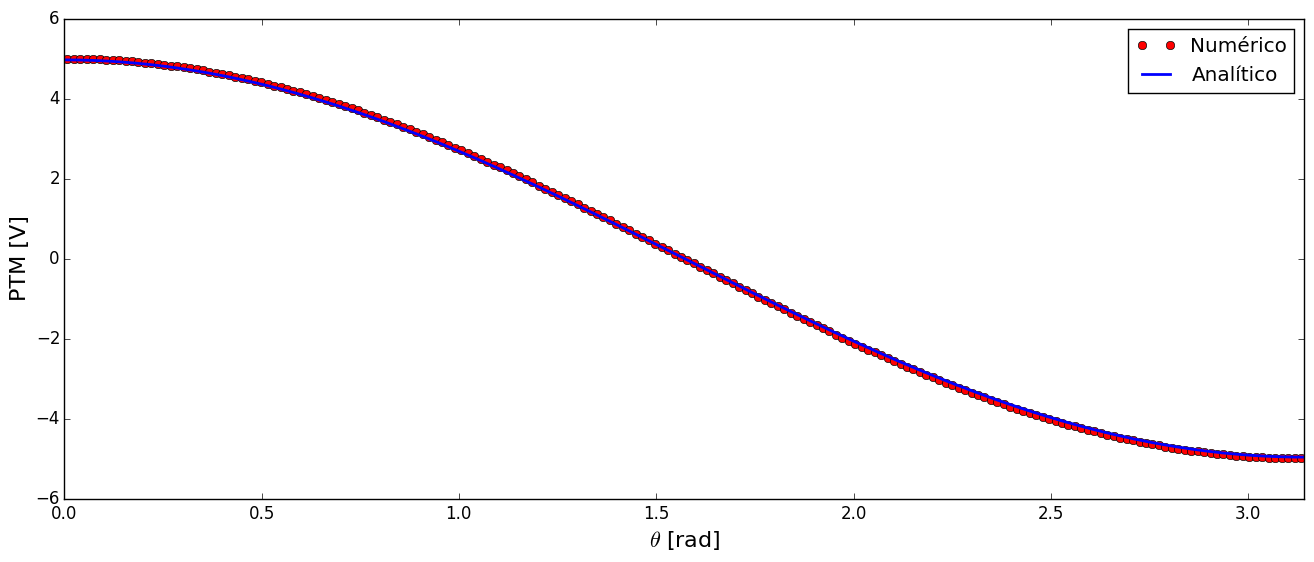
\includegraphics[width=1.0\textwidth]{graficos/itv-vs-teo}}
	E = 1600 \si{\volt\per\centi\metre} y $\alpha$ = 25 \si{\micro\metre}
}

\section{Poros} 

%\subsection{Teoría} 

\frame {
	\frametitle{Generación y evolución de poros en la membrana}
	Densidad de poros:
	\begin{equation*}
		\frac{\partial N}{\partial t} = \alpha_c e^{(PTM/V_{ep})^2} \left( 1 - \frac{N}{N_0 e^{q \left(PTM/V_{ep} \right) ^2}} \right)
	\end{equation*}	\pause
	Radios de los poros:
	\begin{equation*}
		\frac{\partial r}{\partial t} = \frac{D}{kT} \left( \frac{PTM^2 F_{max}}{1+r_h / (r+r_a)} + \frac{4 \beta}{r} \left(\frac{r_*}{r}\right)^4 - 2 \pi \gamma + 2 \pi \sigma_{\textrm{\tiny eff}} r\right)
	\end{equation*} 
	con
	\begin{equation*}
		\sigma_{\textrm{\tiny eff}} = 2 \sigma^\prime - \frac{2 \sigma^\prime - \sigma_0}{(1 - A_p / A)^2}
	\end{equation*}
}

\frame {
	\frametitle{Generación y evolución de poros en la membrana}
	Se asume que la membrana se carga como un capacitor y una resistencia en paralelo:
	\begin{equation*} \begin{split}
		PTM = V_p\, (1 - e^{-t/\tau}) , \\ \textrm{donde } \tau = \alpha\, C_m \left( \frac{1}{\sigma_i} + \frac{1}{2 \sigma_o} \right)
	\end{split} \end{equation*} \pause
	Se actualizan los valores de conductividad de la membrana:
	\begin{equation*} 
		\sigma_{\textrm{\tiny elem}} = \sigma_m (1 - p) + \sigma_p p
	\end{equation*} \pause
	Y se actualizan los valores de difusión de la membrana:
	\begin{equation*} 
		D{\textrm{\tiny elem}} = D_m (1 - p) + D_p p
	\end{equation*}
}

%\subsection{Resultados}

\frame {
	%histogramas. quizás hacer videos de los histogramas?
	%TODO hacer videos de los histogramas
	\frametitle{Densidades de radios para 1200 \si{\volt\per\centi\metre}}
	\begin{multicols}{2}
		\center{En $t = 20$ \si{\micro\second}:}
		\center{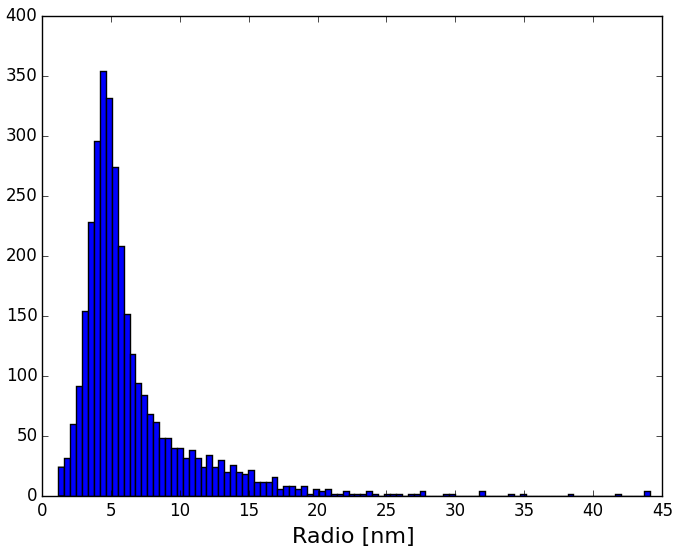
\includegraphics[width=0.50\textwidth]{graficos/poros/120kvm/20micro}}\\
		\columnbreak
		\pause
		\center{En $t = 500$ \si{\micro\second}:}
		\center{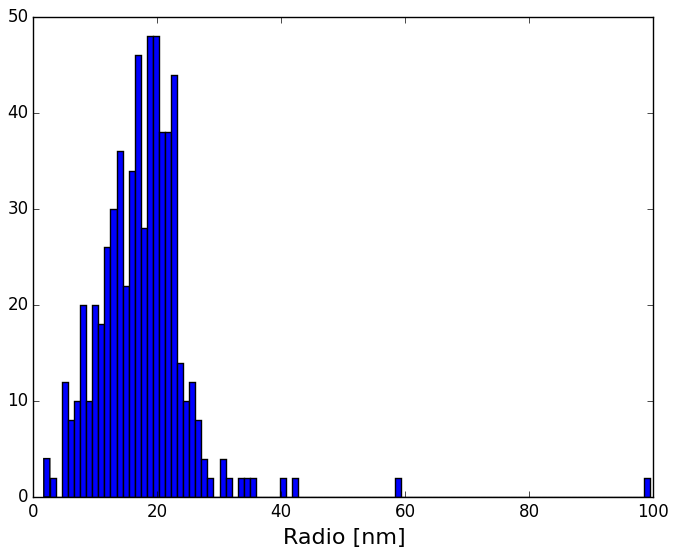
\includegraphics[width=0.50\textwidth]{graficos/poros/120kvm/500micro}}\\
	\end{multicols}
}


\frame {
	\frametitle{Densidades de radios para 1600 \si{\volt\per\centi\metre}}
	\begin{multicols}{2}
		\center{En $t = 20$ \si{\micro\second}:}
		\center{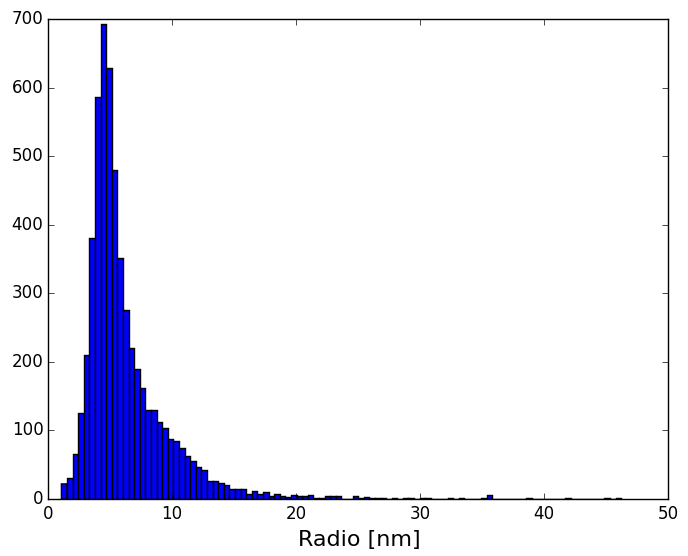
\includegraphics[width=0.50\textwidth]{graficos/poros/160kvm/20micro}}\\
		\columnbreak
		\pause
		\center{En $t = 500$ \si{\micro\second}:}
		\center{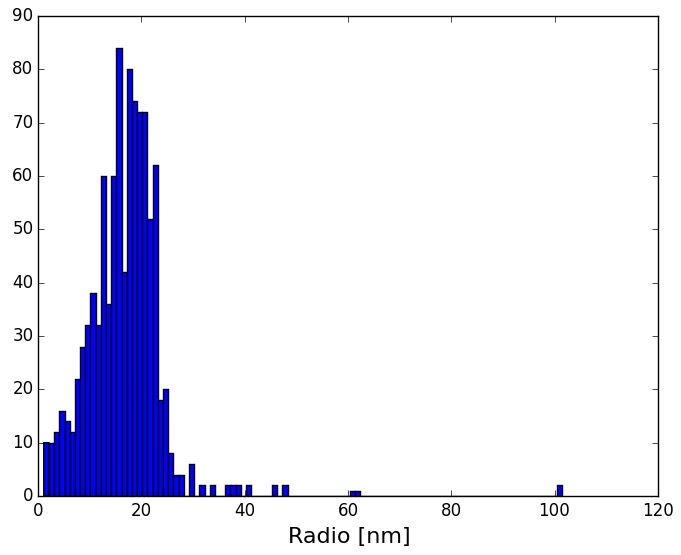
\includegraphics[width=0.50\textwidth]{graficos/poros/160kvm/500micro}}\\
	\end{multicols}
}

\frame {
	\frametitle{Densidades de radios con varios pulsos}
	Para E = 1600 \si{\volt\per\centi\metre} y $\alpha$ = 25 \si{\micro\metre}
	\begin{multicols}{2}
		\center{Primer pulso:}
		\center{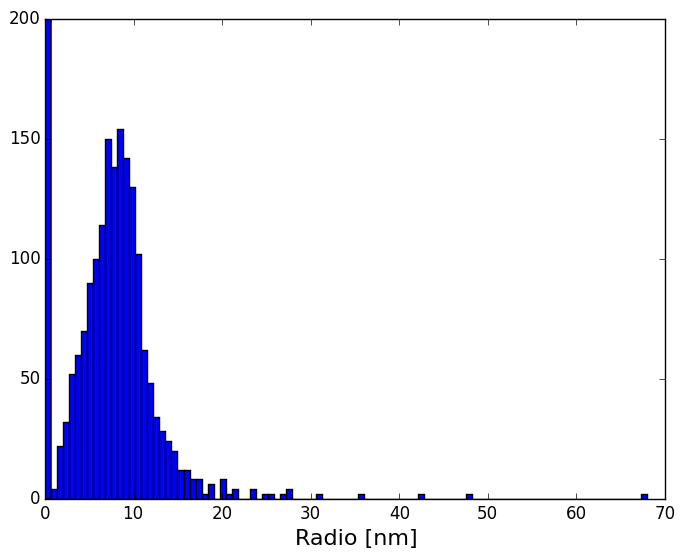
\includegraphics[width=0.50\textwidth]{graficos/poros/160kvm/pulso1}}\\
		\columnbreak
		\pause
		\center{Segundo pulso:}
		\center{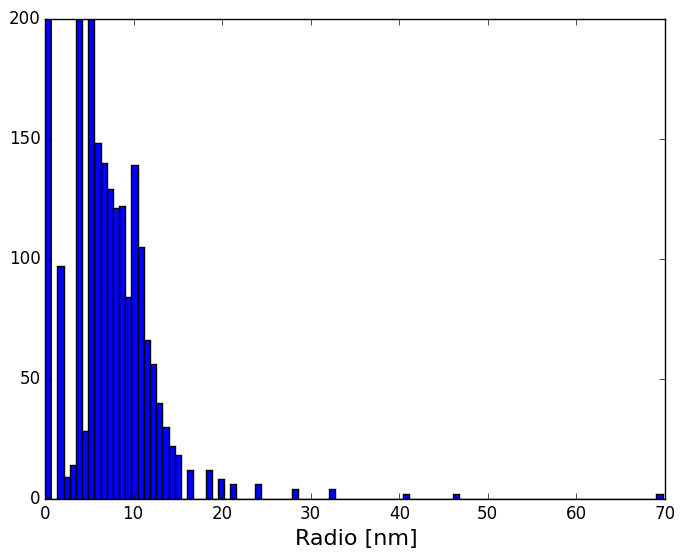
\includegraphics[width=0.50\textwidth]{graficos/poros/160kvm/pulso2}}\\
	\end{multicols}
}

\frame {
	\frametitle{Densidades de radios con varios pulsos}
	\begin{multicols}{2}
		\center{Tercer pulso:}
		\center{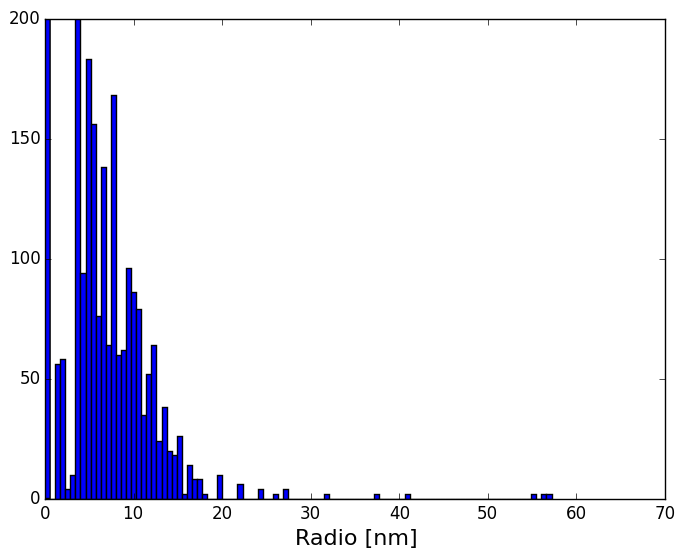
\includegraphics[width=0.50\textwidth]{graficos/poros/160kvm/pulso3}}\\
		\columnbreak
		\pause
		\center{Cuarto pulso:}
		\center{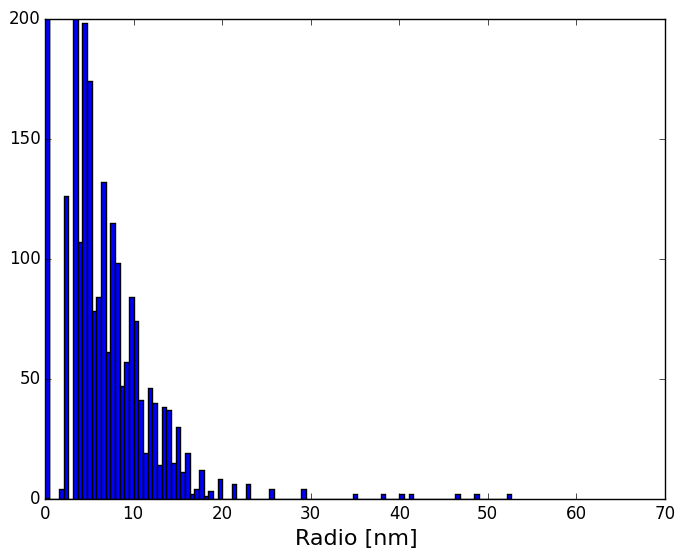
\includegraphics[width=0.50\textwidth]{graficos/poros/160kvm/pulso4}}\\
	\end{multicols}
}

%TODO videos de PTM en función del tiempo

\frame {
	\frametitle{PTM en función del tiempo}
	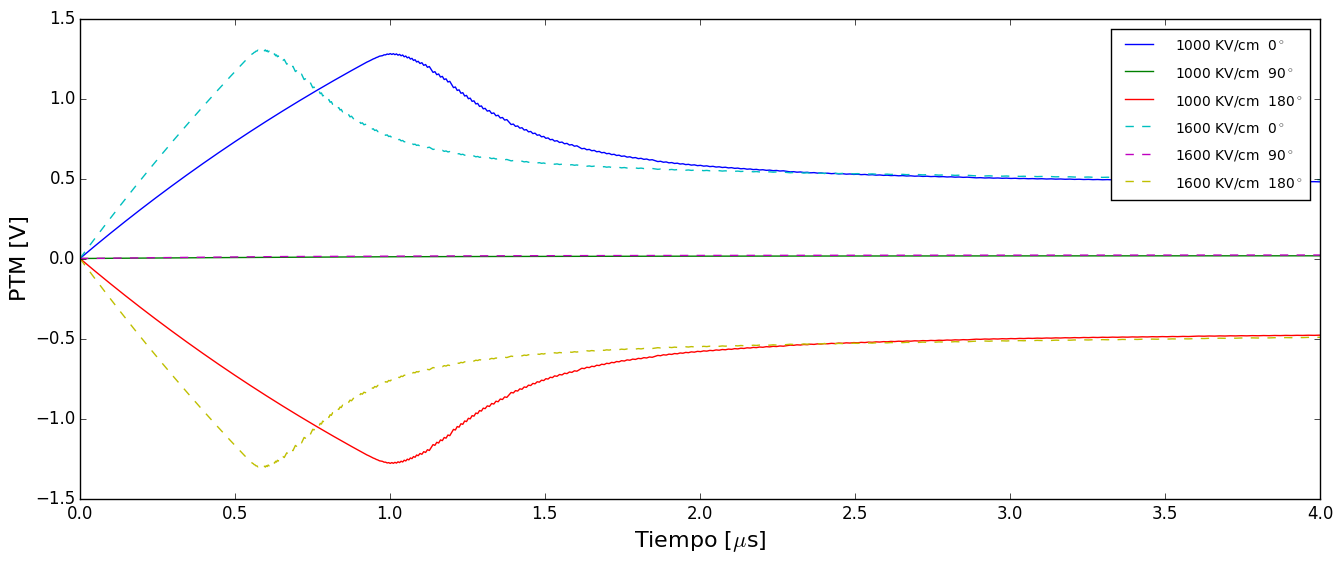
\includegraphics[width=\textwidth]{graficos/poros/itv-time}
}

\frame {
	\frametitle{PTM en función del ángulo polar para E = 1600 \si{\volt\per\centi\metre}}
	\center{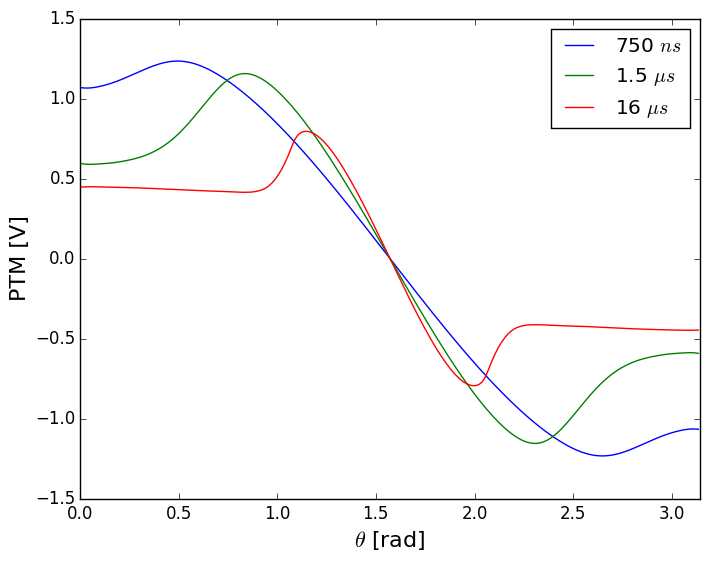
\includegraphics[height=0.85\textheight]{graficos/poros/160kvm/tita}}
}

\section{Transporte}

%\subsection{Teoría} 

\frame {
	\frametitle{Cálculo del transporte de especies en el dominio y a través de la membrana}
	Se sigue la ley de Nernst-Planck:
	\begin{equation*}
		\frac{\partial C_i}{\partial t} = \nabla \cdot \left( D_i \nabla C_i + D_i z_i \frac{F}{R T} C_i \nabla \phi \right)
	\end{equation*}
	Para $i = $ \h, \oh, \na{} ó \cl. \pause
	
	\vspace{2mm}

%Las condiciones de borde son las de dirichlet para los bordes con electrodos. Y las condiciones iniciales a t=0 son valores de esas especies en los tegidos.
%Y pone los valores!!!

	Condiciones de contorno de Dirichlet para los electrodos y Neumann para el borde restante. Concentraciones molares de especies en $t = 0$:

	\vspace{2mm}
	
	\begin{scriptsize} \begin{tabular}{ l | c | c | c | c }
		%\hline
		Especie & \h & \oh & \na & \cl \\
		\hline
  		Interna & \num{.3978e-7} \si{\textsc{m}} & \num{.3978e-7} \si{\textsc{m}} & \num{142} \si{\milli\textsc{m}} & \num{108} \si{\milli\textsc{m}} \\
  		\hline
		Externa & \num{1e-7} \si{\textsc{m}} & \num{1e-7} \si{\textsc{m}} & \num{14e-7} \si{\milli\textsc{m}} & \num{4e-7} \si{\milli\textsc{m}} \\
	\end{tabular} \end{scriptsize}
	
%	\\Condiciones de borde de Dirchlet para los electrodos y de Neumann para el borde no ocupado por los electrodos.
%
%	
%	\vspace{\baselineskip}
%	\\Condiciones de borde de Dirichlet (concentraciones fijas) para $t = 0$ y de Neumann en el borde no ocupado por los electrodos.

}

%\subsection{Resultados} 

\frame {
	\frametitle{Concentraciones}
	Concentraciones para un pulso de 100 \si{\volt\per\centi\metre} en t = 380 \si{\micro\second}
	\begin{multicols}{2}
		\center{\h}
		\center{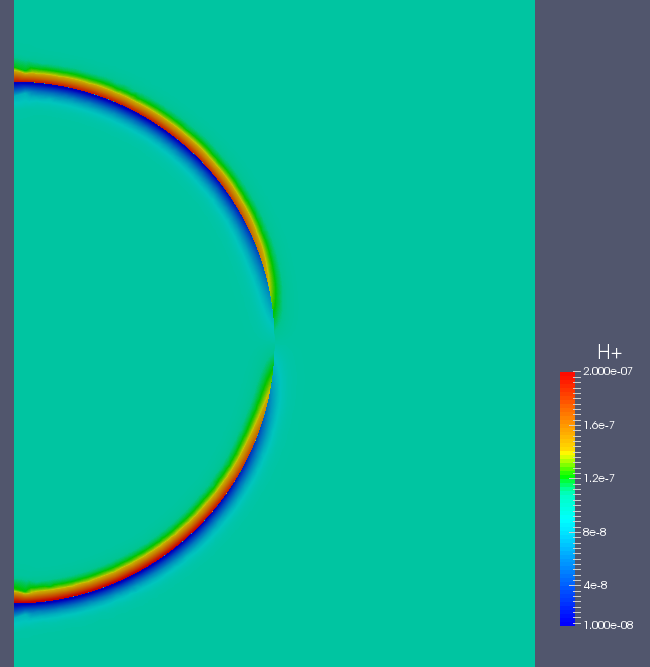
\includegraphics[width=0.50\textwidth]{graficos/trans/h}}\\
		\columnbreak
		\pause
		\center{\oh}
		\center{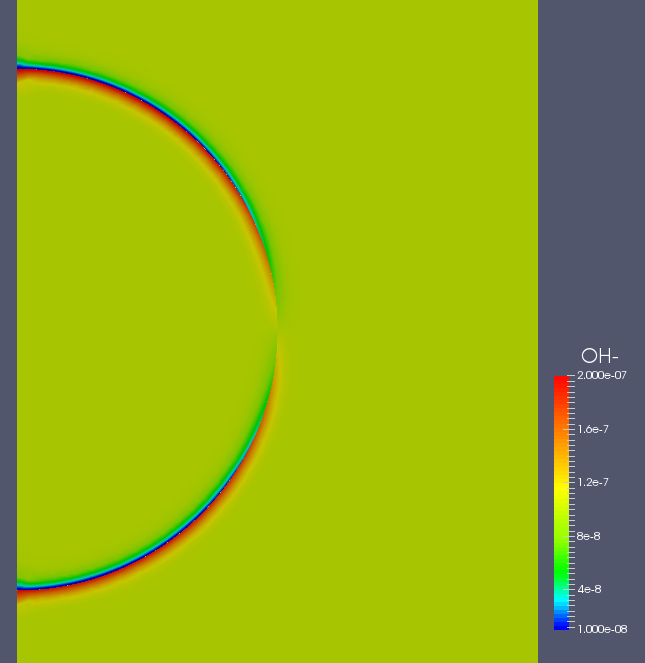
\includegraphics[width=0.50\textwidth]{graficos/trans/oh}}\\
	\end{multicols}
}

%\subsection{Resultados} 

\frame {
	\frametitle{Concentraciones}
	\begin{multicols}{2}
		\center{\na}
		\center{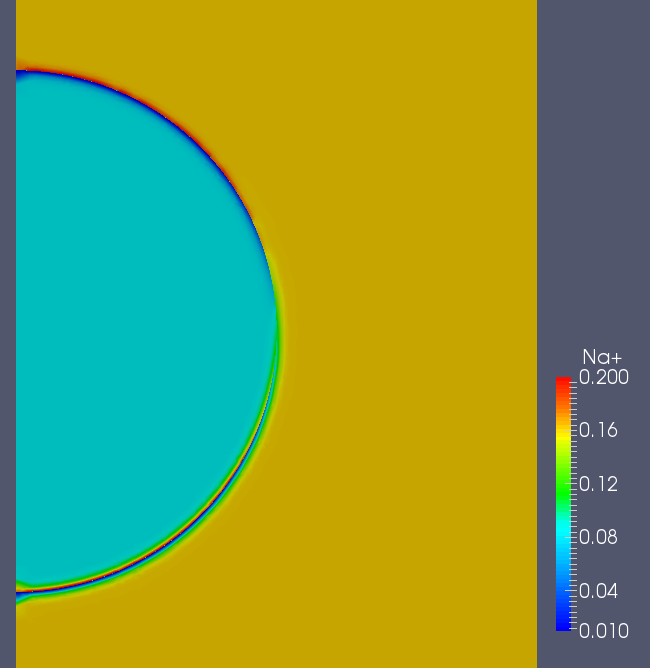
\includegraphics[width=0.50\textwidth]{graficos/trans/na}}\\
		\columnbreak
		\pause
		\center{\cl}
		\center{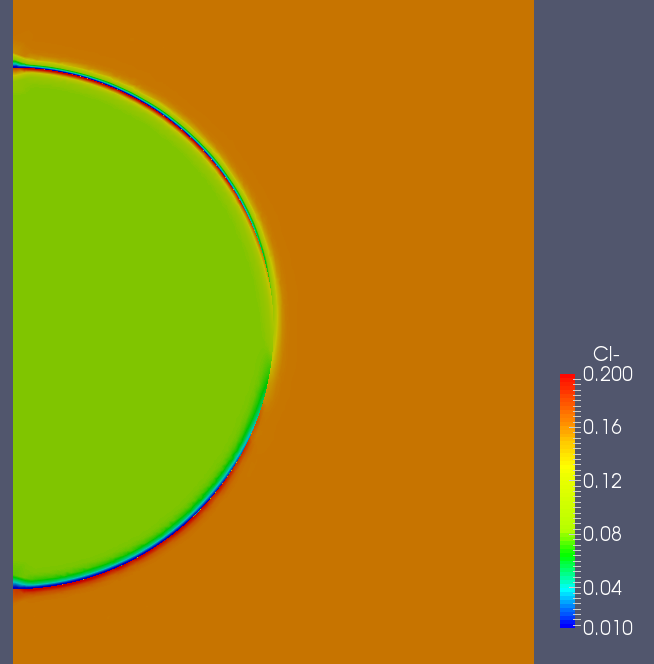
\includegraphics[width=0.50\textwidth]{graficos/trans/cl}}\\
	\end{multicols}
}

\section{Acoplado}

%\subsection{Teoría} 

\frame {
	%Fórmulas. podría ir también un poco de implementación?
	\frametitle{Modelo acoplado}
	Se acoplaron todos los fenómenos físicos anteriores en una sola simulación y se obtuvieron resultados muy diferentes de concentraciones de especies.\\
		
%	6) la 29: Aca pone unos bullets que expliquen las suposiciones principales del modelo acomplado. I) tiempos caracteristicos de cada modelos. II) que se resuelve en cada caso en donde hay potencial aplicado y donde no hay. III) que dato de cada sistema influye en el otro. Por ejemplo el potencial se acompla al modelo de poros al regular apertura y cierre, y el modelo de poros se acopla al trnaporte al regular area de pasaje de especies o apertura de membrana.

	\pause
	\begin{description}
		\item[Poros] Cálculo de población de poros y sus radios individuales, además de cómo afecta las constantes de conductividad y difusión de la membrana celular. Se utiliza un intervalo temporal constante de 1 \si{\nano\second}.
		\item[Potencial] Cálculo del potencial eléctrico en todo el dominio, con un intervalo temporal dinámico: $\Delta_t = 2 \si{\micro\second} \left( 1 - e^{t/-217\si{\nano\second}} \right)$ \pause
		\item[Transporte] Cálculo de las concentraciones de especies en el dominio. Se utiliza un intervalo temporal constante de 200 \si{\nano\second}.
	\end{description}
}

\frame {
	\frametitle{Modelo acoplado}

	\begin{itemize}
		\item El campo eléctrico influye en la creación de poros y en la evolución de sus radios, a través del potencial transmembrana. \pause
		\item Los poros disminuyen la conductividad de la membrana, influyendo en los resultados de campo eléctrico. \pause
		\item El campo eléctrico influye en los resultados de transporte de especies. \pause
		\item Los poros también influyen en el transporte de especies disminuyendo la difusión de la membrana.
	\end{itemize}
}

%\subsection{Concentraciones con un pulso} 

\frame {
	\frametitle{Concentraciones con un pulso}
	%(Videos de concentración un pulso)
	\center { \Huge {
		\href{run:videos/1p/h1.mp4}{\fbox{\parbox[c][1.5cm][c]{0.20\textwidth}{\center{\h}}}}	
		\href{run:videos/1p/oh1.mp4}{\fbox{\parbox[c][1.5cm][c]{0.20\textwidth}{\center{\oh}}}}
		\href{run:videos/1p/na5.mp4}{\fbox{\parbox[c][1.5cm][c]{0.20\textwidth}{\center{\na}}}}
		\href{run:videos/1p/cl1.mp4}{\fbox{\parbox[c][1.5cm][c]{0.20\textwidth}{\center{\cl}}}}
	}}\\
	
	\vspace{2cm}
	Para un pulso de 5 \si{\milli\second} con E = 1600 \si{\volt\per\centi\metre} y $\alpha$ = 25 \si{\micro\metre}
}

%\subsection{Resultados varios pulsos} 

\frame {
	\frametitle{Concentraciones con varios pulsos}
		\center { \Huge {
		\href{run:videos/varios/h1.mp4}{\fbox{\parbox[c][1.5cm][c]{0.20\textwidth}{\center{\h}}}}	
		\href{run:videos/varios/oh2.mp4}{\fbox{\parbox[c][1.5cm][c]{0.20\textwidth}{\center{\oh}}}}
		\href{run:videos/varios/na.mp4}{\fbox{\parbox[c][1.5cm][c]{0.20\textwidth}{\center{\na}}}}
		\href{run:videos/varios/cl1.mp4}{\fbox{\parbox[c][1.5cm][c]{0.20\textwidth}{\center{\cl}}}}
	}}
	
	\vspace{2cm}
	Para 4 pulsos de 5 \si{\milli\second} con E = 1600 \si{\volt\per\centi\metre} y $\alpha$ = 25 \si{\micro\metre}
}

\frame {
	\frametitle{Comparación con resultados experimentales\footfullcite{Biophysical journal, 76(4), 2158-2165, 1999}}
	
	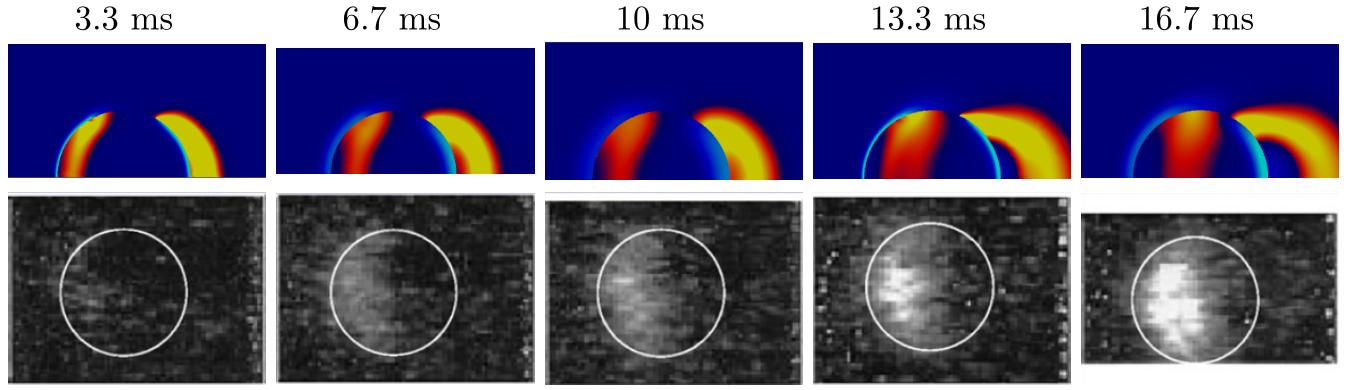
\includegraphics[width=\textwidth]{graficos/experimentales}
}

\section{Escalabilidad}

%\subsection{Escalabilidad} 

\frame {
	\frametitle{Escalabilidad}
	%Mencionar como se usa openmp y resultados
	Se utiliza OpenMP:\pause
	\begin{itemize}
		\item Para llenar en paralelo las matriz usada en el método de elementos finitos para resolver la ecuación de potencial eléctrico. \pause
		\item Para resolver en paralelo las ecuaciones de transporte de las 4 especies iónicas diferentes. \pause
	\end{itemize}
	Resultados de escalabilidad:

	\begin{table}
	    \centering
		\begin{tabular}{ c | c c c c }              
			& 1 thread & 2 threads & 3 threads & 4 threads \\
			\hline
			Tiempo [\si{\second}] & 1995 & 1331 & 1489 & 1233 \\
			Speedup & 1 & 1.50 & 1.34 & 1.63 \\
			Eficiencia & 100\% & 74.9\% & 44.7\% & 40.5\% \\
		\end{tabular}
	    \label{tab:escala}
	\end{table}	
}

\section{Conclusiones} 

%\subsection{Conclusiones} 

\frame {
	\frametitle{Conclusiones}
	\begin{itemize}
		\item El código implementado logra resolver correctamente la dinámica de creación y evolución de poros, la respuesta eléctrica de la célula y el transporte de cuatro especies iónicas, todo esto de manera acoplada. \pause
		\item Se discretizó la membrana explícitamente utilizando un mallado adaptativo, en lugar de considerar la membrana una condición de borde, logrando así resultados que se acercan más a la realidad que los obtenidos en trabajos anteriores. \pause
		\item Se observó el transporte de especies a través de la membrana y se verificó que la apertura de poros contribuye a este fenómeno, ya que se obtuvieron resultados muy diferentes al no considerar electroporación.
	\end{itemize}
}

\frame {
	\frametitle{Conclusiones}
	\begin{itemize}
		\item Se notó claramente que una vez alcanzado un umbral mínimo, aumentar la intensidad del pulso eléctrico no aumenta el potencial transmembrana, pero sí acelera el proceso de permeabilización de la membrana. \pause
		\item Se observó que la mayoría de los poros creados se sellan muy rápidamente, por lo que es necesario repetir el pulso eléctrico periódicamente si se pretende permeabilizar la membrana para introducir especies a la célula.	
	\end{itemize}
}

%\subsection{Trabajo Futuro} 

\frame {
	\frametitle{Trabajo Pendiente}
	\begin{itemize}
		\item Simular distintos tipos de pulsos. \pause
		\item Estudiar un dominio con más de una célula. \pause
		\item Estudiar el efecto de las concentraciones de especies (en especial el pH) sobre las conductividades. \pause
		\item Modelar células irregulares en lugar de esféricas, como las encontradas en los tejidos. \pause
		\item Modelar la deformación de las células producto del campo eléctrico (está siendo realizado en otro trabajo de tesis).
	\end{itemize}
}

\frame {
	\center {\Huge{
		¡Muchas gracias!
	}}
}

\frame {
	\center {\Huge{
		¿Preguntas?
	}}
}

\end{document}
